% Options for packages loaded elsewhere
% Options for packages loaded elsewhere
\PassOptionsToPackage{unicode}{hyperref}
\PassOptionsToPackage{hyphens}{url}
%
\documentclass[
  11pt,
  letterpaper,
  DIV=11,
  numbers=noendperiod,
  twoside]{scrartcl}
\usepackage{xcolor}
\usepackage[left=1.1in, right=1in, top=0.8in, bottom=0.8in,
paperheight=9.5in, paperwidth=7in, includemp=TRUE, marginparwidth=0in,
marginparsep=0in]{geometry}
\usepackage{amsmath,amssymb}
\setcounter{secnumdepth}{3}
\usepackage{iftex}
\ifPDFTeX
  \usepackage[T1]{fontenc}
  \usepackage[utf8]{inputenc}
  \usepackage{textcomp} % provide euro and other symbols
\else % if luatex or xetex
  \usepackage{unicode-math} % this also loads fontspec
  \defaultfontfeatures{Scale=MatchLowercase}
  \defaultfontfeatures[\rmfamily]{Ligatures=TeX,Scale=1}
\fi
\usepackage{lmodern}
\ifPDFTeX\else
  % xetex/luatex font selection
  \setmathfont[]{Garamond-Math}
\fi
% Use upquote if available, for straight quotes in verbatim environments
\IfFileExists{upquote.sty}{\usepackage{upquote}}{}
\IfFileExists{microtype.sty}{% use microtype if available
  \usepackage[]{microtype}
  \UseMicrotypeSet[protrusion]{basicmath} % disable protrusion for tt fonts
}{}
\usepackage{setspace}
% Make \paragraph and \subparagraph free-standing
\makeatletter
\ifx\paragraph\undefined\else
  \let\oldparagraph\paragraph
  \renewcommand{\paragraph}{
    \@ifstar
      \xxxParagraphStar
      \xxxParagraphNoStar
  }
  \newcommand{\xxxParagraphStar}[1]{\oldparagraph*{#1}\mbox{}}
  \newcommand{\xxxParagraphNoStar}[1]{\oldparagraph{#1}\mbox{}}
\fi
\ifx\subparagraph\undefined\else
  \let\oldsubparagraph\subparagraph
  \renewcommand{\subparagraph}{
    \@ifstar
      \xxxSubParagraphStar
      \xxxSubParagraphNoStar
  }
  \newcommand{\xxxSubParagraphStar}[1]{\oldsubparagraph*{#1}\mbox{}}
  \newcommand{\xxxSubParagraphNoStar}[1]{\oldsubparagraph{#1}\mbox{}}
\fi
\makeatother


\usepackage{longtable,booktabs,array}
\usepackage{calc} % for calculating minipage widths
% Correct order of tables after \paragraph or \subparagraph
\usepackage{etoolbox}
\makeatletter
\patchcmd\longtable{\par}{\if@noskipsec\mbox{}\fi\par}{}{}
\makeatother
% Allow footnotes in longtable head/foot
\IfFileExists{footnotehyper.sty}{\usepackage{footnotehyper}}{\usepackage{footnote}}
\makesavenoteenv{longtable}
\usepackage{graphicx}
\makeatletter
\newsavebox\pandoc@box
\newcommand*\pandocbounded[1]{% scales image to fit in text height/width
  \sbox\pandoc@box{#1}%
  \Gscale@div\@tempa{\textheight}{\dimexpr\ht\pandoc@box+\dp\pandoc@box\relax}%
  \Gscale@div\@tempb{\linewidth}{\wd\pandoc@box}%
  \ifdim\@tempb\p@<\@tempa\p@\let\@tempa\@tempb\fi% select the smaller of both
  \ifdim\@tempa\p@<\p@\scalebox{\@tempa}{\usebox\pandoc@box}%
  \else\usebox{\pandoc@box}%
  \fi%
}
% Set default figure placement to htbp
\def\fps@figure{htbp}
\makeatother


% definitions for citeproc citations
\NewDocumentCommand\citeproctext{}{}
\NewDocumentCommand\citeproc{mm}{%
  \begingroup\def\citeproctext{#2}\cite{#1}\endgroup}
\makeatletter
 % allow citations to break across lines
 \let\@cite@ofmt\@firstofone
 % avoid brackets around text for \cite:
 \def\@biblabel#1{}
 \def\@cite#1#2{{#1\if@tempswa , #2\fi}}
\makeatother
\newlength{\cslhangindent}
\setlength{\cslhangindent}{1.5em}
\newlength{\csllabelwidth}
\setlength{\csllabelwidth}{3em}
\newenvironment{CSLReferences}[2] % #1 hanging-indent, #2 entry-spacing
 {\begin{list}{}{%
  \setlength{\itemindent}{0pt}
  \setlength{\leftmargin}{0pt}
  \setlength{\parsep}{0pt}
  % turn on hanging indent if param 1 is 1
  \ifodd #1
   \setlength{\leftmargin}{\cslhangindent}
   \setlength{\itemindent}{-1\cslhangindent}
  \fi
  % set entry spacing
  \setlength{\itemsep}{#2\baselineskip}}}
 {\end{list}}
\usepackage{calc}
\newcommand{\CSLBlock}[1]{\hfill\break\parbox[t]{\linewidth}{\strut\ignorespaces#1\strut}}
\newcommand{\CSLLeftMargin}[1]{\parbox[t]{\csllabelwidth}{\strut#1\strut}}
\newcommand{\CSLRightInline}[1]{\parbox[t]{\linewidth - \csllabelwidth}{\strut#1\strut}}
\newcommand{\CSLIndent}[1]{\hspace{\cslhangindent}#1}



\setlength{\emergencystretch}{3em} % prevent overfull lines

\providecommand{\tightlist}{%
  \setlength{\itemsep}{0pt}\setlength{\parskip}{0pt}}



 


\setlength\heavyrulewidth{0ex}
\setlength\lightrulewidth{0ex}
\usepackage[automark]{scrlayer-scrpage}
\clearpairofpagestyles
\cehead{
  Brian Weatherson
  }
\cohead{
  A Break in the Citation Patterns
  }
\ohead{\bfseries \pagemark}
\cfoot{}
\makeatletter
\newcommand*\NoIndentAfterEnv[1]{%
  \AfterEndEnvironment{#1}{\par\@afterindentfalse\@afterheading}}
\makeatother
\NoIndentAfterEnv{itemize}
\NoIndentAfterEnv{enumerate}
\NoIndentAfterEnv{description}
\NoIndentAfterEnv{quote}
\NoIndentAfterEnv{equation}
\NoIndentAfterEnv{longtable}
\NoIndentAfterEnv{abstract}
\renewenvironment{abstract}
 {\vspace{-1.25cm}
 \quotation\small\noindent\emph{Abstract}:}
 {\endquotation}
\newfontfamily\tfont{EB Garamond}
\addtokomafont{disposition}{\rmfamily}
\addtokomafont{title}{\normalfont\itshape}
\let\footnoterule\relax

\makeatletter
\renewcommand{\@maketitle}{%
  \newpage
  \null
  \vskip 2em%
  \begin{center}%
  \let \footnote \thanks
    {\itshape\huge\@title \par}%
    \vskip 0.5em%  % Reduced from default
    {\large
      \lineskip 0.3em%  % Reduced from default 0.5em
      \begin{tabular}[t]{c}%
        \@author
      \end{tabular}\par}%
    \vskip 0.5em%  % Reduced from default
    {\large \@date}%
  \end{center}%
  \par
  }
\makeatother
\RequirePackage{lettrine}

\renewenvironment{abstract}
 {\quotation\small\noindent\emph{Abstract}:}
 {\endquotation\vspace{-0.02cm}}

\setmainfont{EB Garamond Math}[
  BoldFont = {EB Garamond SemiBold},
  ItalicFont = {EB Garamond Italic},
  RawFeature = {+smcp},
]

\newfontfamily\scfont{EB Garamond Regular}[RawFeature=+smcp]
\renewcommand{\textsc}[1]{{\scfont #1}}

\renewcommand{\LettrineTextFont}{\scfont}
\KOMAoption{captions}{tableheading}
\makeatletter
\@ifpackageloaded{caption}{}{\usepackage{caption}}
\AtBeginDocument{%
\ifdefined\contentsname
  \renewcommand*\contentsname{Table of contents}
\else
  \newcommand\contentsname{Table of contents}
\fi
\ifdefined\listfigurename
  \renewcommand*\listfigurename{List of Figures}
\else
  \newcommand\listfigurename{List of Figures}
\fi
\ifdefined\listtablename
  \renewcommand*\listtablename{List of Tables}
\else
  \newcommand\listtablename{List of Tables}
\fi
\ifdefined\figurename
  \renewcommand*\figurename{Figure}
\else
  \newcommand\figurename{Figure}
\fi
\ifdefined\tablename
  \renewcommand*\tablename{Table}
\else
  \newcommand\tablename{Table}
\fi
}
\@ifpackageloaded{float}{}{\usepackage{float}}
\floatstyle{ruled}
\@ifundefined{c@chapter}{\newfloat{codelisting}{h}{lop}}{\newfloat{codelisting}{h}{lop}[chapter]}
\floatname{codelisting}{Listing}
\newcommand*\listoflistings{\listof{codelisting}{List of Listings}}
\makeatother
\makeatletter
\makeatother
\makeatletter
\@ifpackageloaded{caption}{}{\usepackage{caption}}
\@ifpackageloaded{subcaption}{}{\usepackage{subcaption}}
\makeatother
\usepackage{bookmark}
\IfFileExists{xurl.sty}{\usepackage{xurl}}{} % add URL line breaks if available
\urlstyle{same}
\hypersetup{
  pdftitle={A Break in the Citation Patterns},
  pdfauthor={Brian Weatherson},
  hidelinks,
  pdfcreator={LaTeX via pandoc}}


\title{A Break in the Citation Patterns}
\author{Brian Weatherson}
\date{2024}
\begin{document}
\maketitle
\begin{abstract}
Comments on Eugenio Petrovich's book \emph{A Quantitative Portrait of
Analytic Philosophy: Looking Through the Margins}, for the Quantitative
Studies of Philosophy workshop at Tiburg, August 21-22 2024.
\end{abstract}


\setstretch{1.1}
First, I'd like to thank the organisers for putting on these great
workshops, and Eugenio for writing such a well researched and endlessly
thought provoking book.

I'm going to comment just on one study in the book - the intriguing
suggestion that there's a break in the citation patterns around 2000.
This is intriguing because it connects to a question that's long
interested me: can Late Analytic Philosophy be usefully divided into
eras? Are there periods within Late Analytic that are usefully separated
out from the rest the way it is useful to separate out the Ordinary
Language era, at least in the UK, from the times around it? No such
periodization has caught on, and maybe that's because there isn't a
useful one to find, but if the citations change around 2000, maybe we
should think about whether that's the start of a new era.

The details will matter a bit here, so let me go over what's happening
at this stage of the book (i.e., section 4.4 of the book). We start with
all the citations in five big journals: \emph{Mind}, \emph{Philosophical
Review}, \emph{Journal of Philosophy}, \emph{Noûs} and \emph{Philosophy
and Phenomenological Research}, for each year from 1980-2020. We
represent the citations in each year as a vector, with a dimension for
each article cited at any time in the study, and the magnitude of that
dimension being the number of citations. That gives us 41 n-dimensional
vectors, and we can look at their similarity by taking the cosine of the
angle between them. The result is Figure~\ref{fig-eugenio-matrix}.

\begin{figure}

\centering{

\pandocbounded{\includegraphics[keepaspectratio]{cosine-screenshot.png}}

}

\caption{\label{fig-eugenio-matrix}From page 103 of Petrovich
(\citeproc{ref-Petrovich2024}{2024}).}

\end{figure}%

The darker cells are more similar years, so in the middle of the graph,
we see several years where the similarity scores are relatively high:
around 0.5. Each row of that graph is itself a vector. Eugenio looked
for clusters within those vectors, and Figure~\ref{fig-eugenio-cluster}
shows what he found.

\begin{figure}

\centering{

\pandocbounded{\includegraphics[keepaspectratio]{cluster-screenshot.png}}

}

\caption{\label{fig-eugenio-cluster}From page 103 of Petrovich
(\citeproc{ref-Petrovich2024}{2024}).}

\end{figure}%

In this graph there are three clusters, but the blue cluster to me feels
fairly connected to the green one. What strikes me about this graph is
how few dark cells there are where one year is before 1996 and the other
year is after 1996. Somewhere between 1996 and 2006, there seems to be a
step change here. What could explain that, and does it have a larger
historical significance?

Being old enough to have some memories of this time, I had two thoughts
about what might be going on which I don't think end up being supported
by the data.

One was that there was a change in who the heroes of the narrative were
around then. The giants of the mid twentieth century, particularly
Wittgenstein, Rawls, Quine, and Davidson, seemed to be a smaller part of
the discussion than they had been a few years earlier. But while that
may be reflected in the data for Wittgenstein, the fact that Quine and
Davidson write two of the five pieces most cited in these journals
around the turn of the century doesn't really back up that theory.

A second was that that time was characterised by many more flurries of
interest in particular problems or approaches. Some of these had more
lasting impacts than others, but it was striking how many of them there
were. By the early 2000s, all of these were prominent topics of
conversation, at least around prominent East Coast philosophy
departments, in a way that distinguished that time from earlier or later
times:

\begin{itemize}
\tightlist
\item
  Non-conceptual content
\item
  Zombies
\item
  Fictionalism
\item
  Vagueness
\item
  Self-locating belief (i.e., Sleeping Beauty)
\end{itemize}

But while these were definitely hot topics - at one stage you could
apparently start a conversation with a Princeton grad student by asking
what they were working on fictionalism about - I don't really see them
represented enough in those five journals to make a difference. If we
were looking at \emph{Analysis}, which was much more sensitive to trends
like these, the story might be different. There was a bit on
non-conceptual content, in \emph{Philosophical Review} in particular,
but it probably made the citation record \emph{less} distinctive,
because it connected to earlier discussions by Evans and others. So I
don't think that's the explanation here.

It could be that technological changes around this time, i.e., the rise
of the internet, made a difference. The internet made it somewhat easier
to read articles. It made it much easier to look up citation info, and
so maybe citations that got cut because the author didn't want to trudge
to the library to look up page numbers instead got left in. But I
suspect two other things are more important. It meant philosophers
across long distances could communicate in writing in real time. So
written versions of ideas could spread before they were in print. That
was probably connected to the growth of so many hot topics. And it was
much easier to organise and publicise small workshops and conferences,
especially in the eastern United States. Maybe that's part of the
explanation, though I don't have any direct evidence for it, and I want
to turn to Eugenio's main suggestion for what's going on.

Eugenio suggests that a big part of the story is the rise of
epistemology. If that's the explanation, I suspect that's telling us
something about the sociology of the journals, and of the field, not
about the trends.

There are two important things happen to epistemology around this time.

One is that Ernie Sosa becomes editor of both \emph{Noûs} and
\emph{PPR}. And then those two journals publish more epistemology.

The other is that the boundary between epistemology and philosophy of
science shifts. Some of the most important articles in late twentieth
century epistemology are in philosophy of science journals. Think of ``A
Non-Pragmatic Vindication of Probabilism''
(\citeproc{ref-Joyce1998}{Joyce 1998}), or ``Conditionalizing on
Knowledge''\footnote{This doesn't have a ton of citations, but it is
  reprinted as a key chapter of \emph{Knowledge and Its Limits}}
(\citeproc{ref-Williamson1998}{Williamson 1998}). Around this time the
Formal \textbf{Epistemology} Workshop gets going, pushing the idea that
work that was previously considered part of philosophy of science is now
epistemology.

Between these factors, both pull factors from the editorial changes, and
push factors from the field, I think what we see is a move of
epistemology from specialist journals into `generalist' journals.

It's possible the reverse is happening in political philosophy; those
journals are becoming less important to political philosophy than more
specialist journals like \emph{Ethics} and \emph{Philosophy and Public
Affairs}. There is a discussion to be had here about whether the big
five journals really deserve the name `generalist' in this period, but
I'll leave that for another day.

Because I want to end by sketching a little study I did that might
suggest a different reason for the results in those two figures. I think
they're really telling us something about something strange happening in
the late 1980s and early 1990s. There are a lot fewer `big' articles
from that time. By a big article I mean one that's being \emph{very}
widely cited within a few years, and has a long tail of citations that
persist over decades. Philosophy always has these; except, I think, for
that period. Maybe what's distinctive in the citations around 2000 is
that there should be, but isn't the long tail of articles from 10-15
years earlier (plus/minus a few) that would normally be setting the
agenda.

So far I've said a lot of things that are very vibes based, so let me
give you some data. This is also based on a citation study, and one that
I think complements Eugenio's study. He looked at \textbf{all} the
citations in a \textbf{few} journals. I'm working on a study that flips
that around: I'm looking at a smaller selection of the citations in all
the philosophy journals. The point is not that he did anything wrong and
I'm doing it right. The point is rather, as he says in section 3.4, that
what we're doing here is building \textbf{models} of the field. All
models have strengths and weaknesses; we should build several and see
how they interact.

So what I did was take the Web of Science data, and focus on 100
philosophy journals from 1956 onwards. For each year from 1956-2015 I
made a list of one hundred widely cited articles, with a mix of articles
that were widely cited immediately after publication, articles that have
been widely cited in the last few years, and articles that are widely
cited overall. That gave me 6000 articles. Then I repeated the kind of
analysis Eugenio did, looking at more journals (100 rather than 5), but
with many fewer cited sources (just those 6000 rather than everything).

Figure~\ref{fig-matrix} shows the year by year similarity.

\begin{figure}

\centering{

\pandocbounded{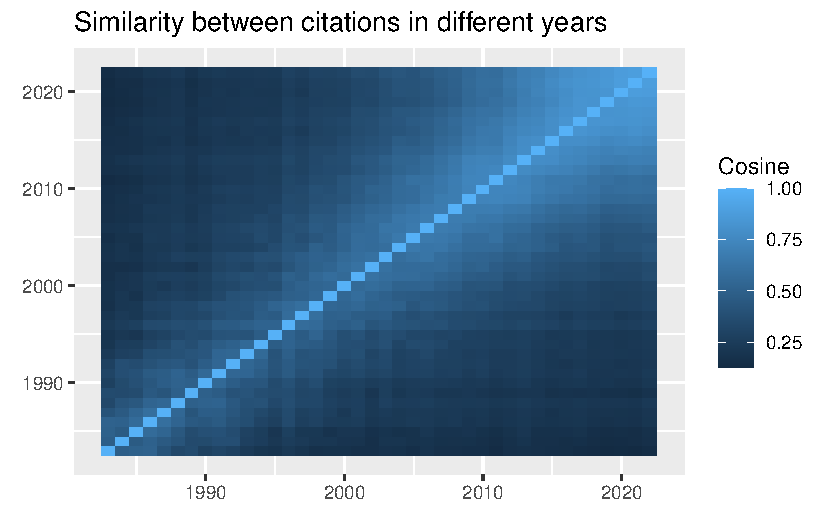
\includegraphics[keepaspectratio]{citation-break_files/figure-pdf/fig-matrix-1.png}}

}

\caption{\label{fig-matrix}Similarity between citations for different
years.}

\end{figure}%

This starts in 1960 because before that, citations to articles published
1956 or later are few enough that it's mostly just noise.

There doesn't seem to be any sharp break around 2000. To see if I was
missing something, for each year I calculated the average of the
similarity measure between it and the preceding five years, and the
result is Figure~\ref{fig-rolling-average}. Again, I've left out the
very noisy years at the very start; the first year here is 1970, so the
first year whose citations get used is 1965

\begin{figure}

\centering{

\pandocbounded{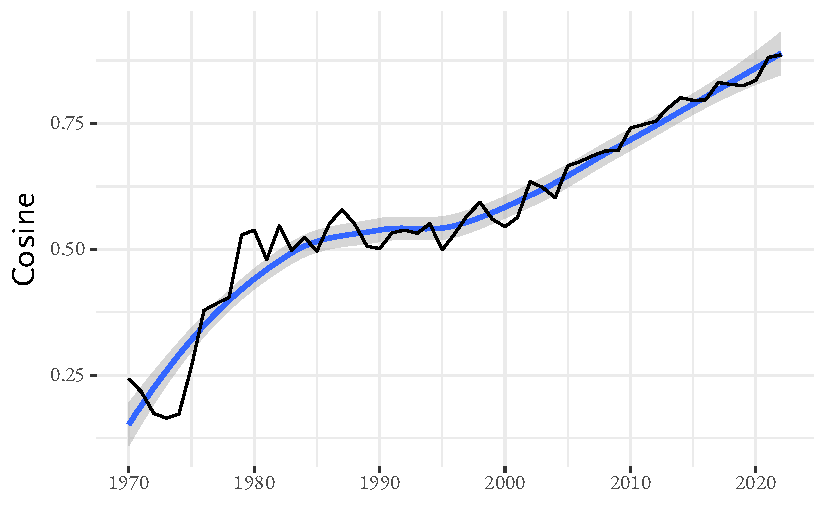
\includegraphics[keepaspectratio]{citation-break_files/figure-pdf/fig-rolling-average-1.pdf}}

}

\caption{\label{fig-rolling-average}Similarity between a year's
citations and the previous five years' citations (1970-2022).}

\end{figure}%

The striking thing in Figure~\ref{fig-rolling-average} is the long pause
between the late 1970s and early 2000s. The trend line even goes gently
down for a while. Given the way I've set things up, that shouldn't
happen. Citations tend to go backwards in time, so each year a new
hundred articles are getting added to the range of possible citations.
That makes a small difference at the end; the new articles are only 2\%
of the universe. But it makes a big difference at the start. So graph,
which measures how similar a year is to the previous 5 in how it treats
these 4000 articles, should slope up. Indeed, if we run the exact same
study starting in 1986 rather than 1956, we get
Figure~\ref{fig-rolling-average-late}, which is what I'd a priori
expect.

\begin{figure}

\centering{

\pandocbounded{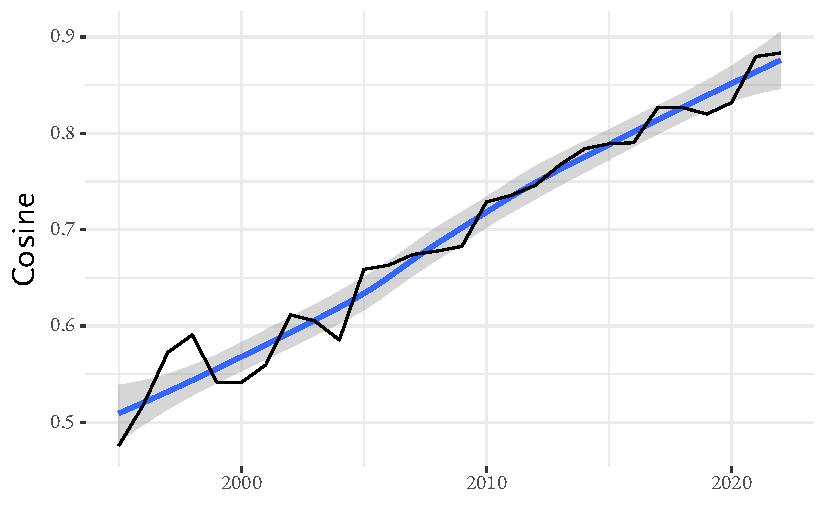
\includegraphics[keepaspectratio]{citation-break_files/figure-pdf/fig-rolling-average-late-1.pdf}}

}

\caption{\label{fig-rolling-average-late}Similarity between a year's
citations and the previous five years' citations (1995-2022).}

\end{figure}%

Something odd is happening with the citations to articles from the 1980s
and early 1990s. Here is my conjecture about why we see something like a
break around 2000. There are three things going on at once.

\begin{enumerate}
\def\labelenumi{\arabic{enumi}.}
\tightlist
\item
  Every year there are a huge number of citations to recently published
  papers; lots of replies, and making small moves on top of recent work.
  These kind of citations keep appearing for a decade or more, but they
  gradually fade away.
\item
  Typically, there are a handful of papers that really define a field,
  and while they aren't always immediately recognised as such, they tend
  to keep being cited, in massive volumes, for many years after the
  fact.
\item
  The 1980s saw fewer of these papers being produced, especially after
  1983. So around 2000 the usual turnover of citations, the allure of
  the new, had a more dramatic effect because it wasn't mixed with
  continued discussion of the field defining papers from 10-15 years
  earlier.
\end{enumerate}

Note here that I'm only making a claim about journal articles. There
were some field defining books published in this time, notably \emph{On
the Plurality of Worlds}. And I haven't done a study of chapters in
edited volumes. But the journals stopped producing articles that had
much staying power. Here's one way to see this.

Start by looking at articles published in the first half of the 2000s,
i.e., 2000-2004. By the end of the 2000s, the 15 most cited articles
from the first half of the decade were shown in
Table~\ref{tbl-early-2000s}.

\begin{longtable}[]{@{}
  >{\raggedright\arraybackslash}p{(\linewidth - 2\tabcolsep) * \real{0.9346}}
  >{\raggedleft\arraybackslash}p{(\linewidth - 2\tabcolsep) * \real{0.0654}}@{}}

\caption{\label{tbl-early-2000s}Most cited 2000s articles by 2009.}

\tabularnewline

\toprule\noalign{}
\begin{minipage}[b]{\linewidth}\raggedright
Article
\end{minipage} & \begin{minipage}[b]{\linewidth}\raggedleft
Citations
\end{minipage} \\
\midrule\noalign{}
\endhead
\bottomrule\noalign{}
\endlastfoot
P Machamer, L Darden, and CF Craver (2000) ``Thinking About
Mechanisms,'' \emph{Philosophy Of Science} 67~(1):~1-25. & 86 \\
W Rabinowicz and T Ronnow-Rasmussen (2004) ``The Strike of the Demon: On
Fitting Pro-Attitudes and Value,'' \emph{Ethics} 114~(3):~391-423. &
71 \\
K DeRose (2003) ``Assertion, Knowledge, and Context,''
\emph{Philosophical Review} 111~(2):~167-203. & 67 \\
J Knobe (2003) ``Intentional Action and Side Effects in Ordinary
Language,'' \emph{Analysis} 63~(3):~190-194. & 58 \\
D Lewis (2000) ``Causation as Influence,'' \emph{Journal Of Philosophy}
97~(4):~182-197. & 57 \\
C Travis (2004) ``The Silence of the Senses,'' \emph{Mind}
113~(449):~57-94. & 55 \\
DJ Chalmers and F Jackson (2001) ``Conceptual Analysis and Reductive
Explanation,'' \emph{Philosophical Review} 110~(3):~315-360. & 54 \\
J Stanley and T Williamson (2001) ``Knowing How,'' \emph{Journal Of
Philosophy} 98~(8):~411-444. & 53 \\
S Glennan (2002) ``Rethinking Mechanistic Explanation,''
\emph{Philosophy Of Science} 69~(3):~342-353. & 46 \\
J Pryor (2000) ``The Skeptic and the Dogmatist,'' \emph{Noûs}
34~(4):~517-549. & 45 \\
M Matthen and A Ariew (2002) ``Two Ways of Thinking About Fitness and
Natural Selection,'' \emph{Journal Of Philosophy} 99~(2):~55-83. & 43 \\
D Pitt (2004) ``The Phenomenology of Cognition, Or, What is It Like To
Think That P?,'' \emph{Philosophy And Phenomenological Research}
69~(1):~1-36. & 43 \\
J MacFarlane (2003) ``Future Contingents and Relative Truth,''
\emph{Philosophical Quarterly} 53~(212):~321-336. & 41 \\
J Schaffer (2003) ``Is There a Fundamental Level?,'' \emph{Noûs}
37~(3):~498-517. & 39 \\
A Hájek (2003) ``What Conditional Probability Could Not Be,''
\emph{Synthese} 137~(3):~273-323. & 39 \\

\end{longtable}

In the most recent 5 years in the available data, 2018-2022,
Table~\ref{tbl-late-2000s} are the most cited articles first published
in 2000-2004.

\begin{longtable}[]{@{}
  >{\raggedright\arraybackslash}p{(\linewidth - 2\tabcolsep) * \real{0.9387}}
  >{\raggedleft\arraybackslash}p{(\linewidth - 2\tabcolsep) * \real{0.0613}}@{}}

\caption{\label{tbl-late-2000s}Most cited 2000s articles since 2018.}

\tabularnewline

\toprule\noalign{}
\begin{minipage}[b]{\linewidth}\raggedright
Article
\end{minipage} & \begin{minipage}[b]{\linewidth}\raggedleft
Citations
\end{minipage} \\
\midrule\noalign{}
\endhead
\bottomrule\noalign{}
\endlastfoot
P Machamer, L Darden, and CF Craver (2000) ``Thinking About
Mechanisms,'' \emph{Philosophy Of Science} 67~(1):~1-25. & 192 \\
S Haslanger (2000) ``Gender and Race: (What) Are They? (What) Do We Want
Them To Be?,'' \emph{Noûs} 34~(1):~31-55. & 182 \\
J Pryor (2000) ``The Skeptic and the Dogmatist,'' \emph{Noûs}
34~(4):~517-549. & 151 \\
J D'Arms and D Jacobson (2000) ``The Moralistic Fallacy: On the
`Appropriateness' of Emotions,'' \emph{Philosophy And Phenomenological
Research} 61~(1):~65-90. & 109 \\
J Stanley and T Williamson (2001) ``Knowing How,'' \emph{Journal Of
Philosophy} 98~(8):~411-444. & 109 \\
H Douglas (2000) ``Inductive Risk and Values in Science,''
\emph{Philosophy Of Science} 67~(4):~559-579. & 96 \\
J Fantl and M McGrath (2002) ``Evidence, Pragmatics, and
Justification,'' \emph{Philosophical Review} 111~(1):~67-94. & 90 \\
AI Goldman (2001) ``Experts: Which Ones Should You Trust?,''
\emph{Philosophy And Phenomenological Research} 63~(1):~85-110. & 89 \\
MGF Martin (2004) ``The Limits of Self-Awareness,'' \emph{Philosophical
Studies} 120~(1-3):~37-89. & 80 \\
K DeRose (2003) ``Assertion, Knowledge, and Context,''
\emph{Philosophical Review} 111~(2):~167-203. & 75 \\
D Lewis (2000) ``Causation as Influence,'' \emph{Journal Of Philosophy}
97~(4):~182-197. & 73 \\
T Kelly (2003) ``Epistemic Rationality as Instrumental Rationality: A
Critique,'' \emph{Philosophy And Phenomenological Research}
66~(3):~612-640. & 70 \\
R Feldman (2000) ``The Ethics of Belief,'' \emph{Philosophy And
Phenomenological Research} 60~(3):~667-695. & 69 \\
W Rabinowicz and T Ronnow-Rasmussen (2004) ``The Strike of the Demon: On
Fitting Pro-Attitudes and Value,'' \emph{Ethics} 114~(3):~391-423. &
69 \\
C Travis (2004) ``The Silence of the Senses,'' \emph{Mind}
113~(449):~57-94. & 65 \\

\end{longtable}

There is a lot of overlap between Table~\ref{tbl-early-2000s} and
Table~\ref{tbl-late-2000s}. In particular, the articles by Peter
Machamer, Lindley Darden, and Carl F. Craver, Wlodek Rabinowicz and Toni
Rønnow‐Rasmussen, Keith DeRose, David Lewis, Charles Travis, Jason
Stanley and Timothy Williamson, and James Pryor are in both lists.
Having 7 articles in both lists like that isn't particularly unusual.

I've used decades to set this up, but really what I did was take some
year \emph{y}, in this case 2000, focus on articles published between
\emph{y} and \emph{y}+4, and compare two lists: which of those articles
were in the 15 most cited before \emph{y}+9, and which were in the 15
most cited between 2018 and 2022. If you do that for different values of
\emph{y}, you often find 5-7 articles in both lists. But if you set
\emph{y} to 1984, so that it focuses on the mid-to-late 1980s, there is
very little overlap. Table~\ref{tbl-early-1980s} lists the articles from
1984-1988 that were most cited by 1993.

\begin{longtable}[]{@{}
  >{\raggedright\arraybackslash}p{(\linewidth - 2\tabcolsep) * \real{0.9301}}
  >{\raggedleft\arraybackslash}p{(\linewidth - 2\tabcolsep) * \real{0.0699}}@{}}

\caption{\label{tbl-early-1980s}Most cited 1984-1988 articles by 1993.}

\tabularnewline

\toprule\noalign{}
\begin{minipage}[b]{\linewidth}\raggedright
Article
\end{minipage} & \begin{minipage}[b]{\linewidth}\raggedleft
Citations
\end{minipage} \\
\midrule\noalign{}
\endhead
\bottomrule\noalign{}
\endlastfoot
T Burge (1986) ``Individualism and Psychology,'' \emph{Philosophical
Review} 95~(1):~3-45. & 47 \\
J Kim (1984) ``Concepts of Supervenience,'' \emph{Philosophy And
Phenomenological Research} 45~(2):~153-176. & 43 \\
J Rawls (1985) ``Justice as Fairness: Political Not Metaphysical,''
\emph{Philosophy \& Public Affairs} 14~(3):~223-251. & 38 \\
P Railton (1986) ``Moral Realism,'' \emph{Philosophical Review}
95~(2):~163-207. & 33 \\
F Jackson and P Pettit (1988) ``Functionalism and Broad Content,''
\emph{Mind} 97~(387):~381-400. & 28 \\
L Laudan (1987) ``Progress or Rationality: The Prospects for Normative
Naturalism,'' \emph{American Philosophical Quarterly} 24~(1):~19-31. &
25 \\
A Baier (1986) ``Trust and Antitrust,'' \emph{Ethics} 96~(2):~231-260. &
21 \\
J Rawls (1988) ``The Priority of Right and Ideas of the Good,''
\emph{Philosophy \& Public Affairs} 17~(4):~251-276. & 21 \\
T Burge (1988) ``Individualism and Self-Knowledge,'' \emph{Journal Of
Philosophy} 85~(11):~649-663. & 21 \\
PM Churchland (1985) ``Reduction, Qualia, and the Direct Introspection
of Brain States,'' \emph{Journal Of Philosophy} 82~(1):~8-28. & 20 \\
RG Millikan (1986) ``Thoughts Without Laws, Cognitive Science With
Content,'' \emph{Philosophical Review} 95~(1):~47-80. & 20 \\
J Bigelow and R Pargetter (1987) ``Functions,'' \emph{Journal Of
Philosophy} 84~(4):~181-196. & 20 \\
P Railton (1984) ``Alienation, Consequentialism, and the Demands of
Morality,'' \emph{Philosophy \& Public Affairs} 13~(2):~134-171. & 19 \\
P Kitcher (1984) ``Species,'' \emph{Philosophy Of Science}
51~(2):~308-333. & 19 \\
R Feldman (1985) ``Reliability and Justification,'' \emph{Monist}
68~(2):~159-174. & 19 \\

\end{longtable}

And Table~\ref{tbl-late-1980s} shows the almost completely distinct list
of articles from 1984 to 1988 that have been widely cited in the last 5
years of the data set.

\begin{longtable}[]{@{}
  >{\raggedright\arraybackslash}p{(\linewidth - 2\tabcolsep) * \real{0.9324}}
  >{\raggedleft\arraybackslash}p{(\linewidth - 2\tabcolsep) * \real{0.0676}}@{}}

\caption{\label{tbl-late-1980s}Most cited 1984-1988 articles since
2018.}

\tabularnewline

\toprule\noalign{}
\begin{minipage}[b]{\linewidth}\raggedright
Article
\end{minipage} & \begin{minipage}[b]{\linewidth}\raggedleft
Citations
\end{minipage} \\
\midrule\noalign{}
\endhead
\bottomrule\noalign{}
\endlastfoot
D Lewis (1984) ``Putnam's Paradox,'' \emph{Australasian Journal Of
Philosophy} 62~(3):~221-236. & 80 \\
P Railton (1984) ``Alienation, Consequentialism, and the Demands of
Morality,'' \emph{Philosophy \& Public Affairs} 13~(2):~134-171. & 73 \\
R Feldman and E Conee (1985) ``Evidentialism,'' \emph{Philosophical
Studies} 48~(1):~15-34. & 70 \\
A Baier (1986) ``Trust and Antitrust,'' \emph{Ethics} 96~(2):~231-260. &
68 \\
G Boolos (1984) ``To Be is To Be a Value of a Variable (Or To Be Some
Values of Some Variables),'' \emph{Journal Of Philosophy}
81~(8):~430-449. & 60 \\
E McMullin (1985) ``Galilean Idealization,'' \emph{Studies In History
And Philosophy Of Science} 16~(3):~247-273. & 59 \\
P Railton (1986) ``Moral Realism,'' \emph{Philosophical Review}
95~(2):~163-207. & 58 \\
J Bogen and J Woodward (1988) ``Saving the Phenomena,''
\emph{Philosophical Review} 97~(3):~303-352. & 57 \\
V McGee (1985) ``A Counterexample To Modus Ponens,'' \emph{Journal Of
Philosophy} 82~(9):~462-471. & 56 \\
S Cohen (1984) ``Justification and Truth,'' \emph{Philosophical Studies}
46~(3):~279-295. & 53 \\
J Hardwig (1985) ``Epistemic Dependence,'' \emph{Journal Of Philosophy}
82~(7):~335-349. & 53 \\
BC van Fraassen (1984) ``Belief and the Will,'' \emph{Journal Of
Philosophy} 81~(5):~235-256. & 51 \\
H Frankfurt (1987) ``Equality as a Moral Ideal,'' \emph{Ethics}
98~(1):~21-43. & 37 \\
W Sinnottarmstrong (1984) ``Ought Conversationally Implies Can,''
\emph{Philosophical Review} 93~(2):~249-261. & 33 \\
F Jackson and R Pargetter (1986) ``Oughts, Options, and Actualism,''
\emph{Philosophical Review} 95~(2):~233-255. & 33 \\

\end{longtable}

Articles from the 1980s that made a big impact at the time were, for the
most part, not sticking around. In part I think that's because the
1980s, or at least the parts that were impactful at the time, were more
`normal science'. There were a lot of articles that tried to make small
improvements, especially on questions surrounding supervenience and
physicalism, and there just wasn't much reason to cite those 15 or so
years late. Maybe the absence of the articles from a decade or so ago
that would normally be cited is part of why there's a break around the
2000s. But this is all speculative, and I think the whole question is
both really interesting, and in need of further study.

So I'll end where I started by saying how grateful I am to the
organisers for putting this on, and to Eugenio for the book. What I've
done here is look at a few things inspired by one section of the book -
it is full of so many insights and observations and it both makes you
rethink what you thought about recent philosophy, and raises many
fascinating questions like the one I've been discussing. I hope it gets
very widely read.

\section*{References}\label{references}
\addcontentsline{toc}{section}{References}

\phantomsection\label{refs}
\begin{CSLReferences}{1}{0}
\bibitem[\citeproctext]{ref-Joyce1998}
Joyce, James M. 1998. {``A Non-Pragmatic Vindication of Probabilism.''}
\emph{Philosophy of Science} 65 (4): 575--603. doi:
\href{https://doi.org/10.1086/392661}{10.1086/392661}.

\bibitem[\citeproctext]{ref-Petrovich2024}
Petrovich, Eugenio. 2024. \emph{A Quantitative Portrait of Analytic
Philosophy: Looking Through the Margins}. Cham: Springer.

\bibitem[\citeproctext]{ref-Williamson1998}
Williamson, Timothy. 1998. {``Conditionalizing on Knowledge.''}
\emph{The British Journal for the Philosophy of Science} 49 (1):
89--121. doi:
\href{https://doi.org/10.1093/bjps/49.1.89}{10.1093/bjps/49.1.89}.

\end{CSLReferences}



\noindent Published online in June 2024.


\end{document}
